

\section{Weighted automata and expressions over free monoids}
\label{sec:aut-fre-mul}


The following functions concern automata over a free monoid --- as 
opposed to automata over a direct product of free monoids.
Their behaviours are series over~$\Ae$, \ie weighted subsets 
of~$\Ae$. 
% 
\Apriori, there is no assumption on the multiplicity (or weight) semiring.
However, in \vcsnv, \tafkit gives access to automata with weight in 
`numerical' \emph{commutative} semirings only.

The next two sections, \secti{aut-fre-fld} and \secti{aut-fre-boo},
will describe functions that are special to 
automata with multiplicity in a field ($\R$, $\Q$ and~$\F_{2}$) and in~$\B$ respectively.


\renewcommand{\theenumii}{\theenumi.\arabic{enumii}}

\begin{enumerate}
       

\item Properties and transformations of automata 

\begin{enumerate}
% \item \Fctaut{is-letterized}, \Fctaut{letterize} 
\item \Fctaut{transpose}
\item \Fctaut{is-realtime}\vrglst \Fctaut{realtime}
\item \Fctaut{is-unambiguous}
\item \Fctaut{partial-identity}\vrglst \Fctaut{partial-erase}
% \item \Fctaut{partial-erase}
\item \Fctaut{characteristic}
\item \Fctaut{support}
% \item \Fctexp{is-letterized-E}, \Fctexp{letterize-E}
\end{enumerate}

\item Behaviour of automata 

\begin{enumerate}
\item \FctParD{eval}{aut}{word}
\item \FctParD{eval-S}{aut}{word}
% \item \Fctaut{shortest}
% \item \FctParD{enumerate}{aut}{n}
\end{enumerate}

\item From expressions to automata

\begin{enumerate}
\item \Fctexp{standard}
\item \Fctexp{thompson}
\item \Fct{alphabet}\vrglst \Fct{star-alphabet}
% \item \Fct{star-alphabet}
% \item \Fctexp{derived-term}
\end{enumerate}

\item Operations on automata

\begin{enumerate}
\item \Fctaut{quotient}\vrglst \Fctaut{coquotient}
\item \FctautD{product}
\item \FctParD{power}{aut}{n}
\item \FctautD{shuffle}\vrglst \FctautD{infiltration}
% \item \FctautD{infiltration}
\end{enumerate}

% \item Operations on behaviours of automata (commutative multiplicity semiring)
% 
% \begin{enumerate}
% \item \FctautD{hadamard-S}
% \item \FctautD{shuffle-S}, \FctautD{infiltration-S}
% \end{enumerate}

\end{enumerate}

\longonly{%
\begin{ComV}%{101205}
    
    \thi not implemented:
%     
    \Fct{is-letterized}, \Fct{letterize}; 

	\Fct{hadamard-S}, \Fct{shuffle-S}, \Fct{infiltration-S};

    the \code{co} commands: \Fct{coquotient}.
    
    \thii transfered to other sections:
%     
    \Fct{derived-term};
	
    \Fct{shortest}, \Fct{enumerate}.
	
	\thiii there is no reason why \Fct{charasteristic} or 
	\Fct{support} should not be called for \fmpts, but they are not...

\end{ComV}
}%

\subsection{Properties and transformations of automata}
\label{aut-mul-tra}%

The following function is not implemented. It is 
just convenient to \emph{describe the specification} of \Fct{realtime}. 

\begin{SwClCmd}
\begin{shell}
$ \kbd{vcsn letterize a.xml > b.xml}
$
\end{shell}%
\end{SwClCmd}%
\begin{SwClTxt}
    Computes from \Prm{a.xml} an equivalent automaton whose 
    transitions are all labelled by letters or the empty word, by  
    cutting the label of every transition into letters and writes the 
    result in \Prm{b.xml}.
\end{SwClTxt}%
\IndexFct{letterize}

\subsubsection{\Fct{transpose}}
\label{ssc:aut-tra}%

\begin{SwClCmd}
\begin{shell}
$ \kbd{vcsn transpose a.xml > b.xml}
$
\end{shell}%
\end{SwClCmd}%
\begin{SwClTxt}
    Computes the transposition of the automaton 
    \Prm{a.xml} and writes the result in \Prm{b.xml}.
\end{SwClTxt}%
\IndexFct{transpose}%


\Spec
Builds the transposition of the underlying graph, 
and  \emph{exchanges} the initial and final functions,
that is, realises the function \Fct{reverse} (\cf 
\secti{aut-fct}).
Finally, transposes 
the labels as well, that is, takes the \emph{mirror} image of the 
words that label the transitions \emph{and} 
\index{condition!scalar end-function}
in the initial and final functions.\footnote{%
   Such automata cannot be built by the \Fct{edit} function
   and will not be considered within \tafkitv (scalar end-function 
   condition).}

\Comt
\thi
The behaviour of~$\jsTrsp{\Ac}$, the tranpose of~$\Ac$, is the 
transpose of the behaviour of~$\Ac$.

\thii 
There exists a \Fct{transpose} function for transducers (\code{fmp}) as 
well, that will be redefined explicitely for them (\cf 
\sbsct{fmp-tra}).


\subsubsection{\Fct{is-realtime}, \Fct{realtime}}
\label{ssc:aut-mul-rea}%

\begin{SwClCmd}
\begin{shell}
$ \kbd{vcsn is-realtime -v a.xml}
Input is realtime
\end{shell}%
\end{SwClCmd}%
\begin{SwClTxt}
    Tells whether or not the automaton 
       \Prm{a.xml} is realtime.
\end{SwClTxt}%
\IndexFctIs{realtime}

\Spec
An automaton (over a free monoid) is realtime if it is both letterized 
and proper.

\Cave
The label of a transition of a realtime automaton is not necessarily 
a weighted letter but may be a \emph{sum} of weighted letters as 
shown on the following example (\cf \figur{c1} for the 
automaton~\code{c1.xml}). 
\begin{shell}
$ \kbd{vcsn-char-z -v is-realtime c1.xml}
Input is realtime
\end{shell}%

% \medskip
\begin{SwClCmd}
\begin{shell}
$ \kbd{vcsn realtime a.xml > b.xml}
$
\end{shell}%
\end{SwClCmd}%
\begin{SwClTxt}
    Computes from \Prm{a.xml} an automaton by
    eliminating the spontaneous transitions from the letterized version 
    of \Prm{a.xml} and writes the result in \Prm{b.xml}.
\end{SwClTxt}%
\IndexFct{realtime}


\Spec
\Fctq{realtime}{a.xml} = 
\Fctq{proper}{\Fctq{letterize}{a.xml}}

\Comt
\thi The problem with \Fct{realtime} is the same as the one of \Fct{proper} and 
has been mentioned at \sbsct{aut-pro}.

\thii \Fctq{letterize}{\Fctq{proper}{a.xml}}
is another realtime automaton, which has potentially (many) more states 
and transitions than \Fctq{realtime}{a.xml}.


\subsubsection{\Fct{is-unambiguous}}

\begin{SwClCmd}
\begin{shell}
$ \kbd{vcsn -v is-unambiguous a.xml}
Input is unambiguous
\end{shell}%
\end{SwClCmd}%
\begin{SwClTxt}
    Tells whether or not the automaton 
    \Prm{a.xml} is unambiguous.
\end{SwClTxt}%
\IndexFct{is-unambiguous}

\Prec
\Prm{a.xml} is a \emph{realtime} automaton.

\Spec 
An automaton is \emph{unambiguous} if every word accepted by the 
automaton is the label of \emph{only one} successful computation. 
\index{automaton!unambiguous}%

\Comt
\thi  Being ambiguous or unambiguous is classically a property of 
Boolean automata. We have found interesting to extend the definition 
to any weighted automata

\thii The function implements the following characterization of 
unambiguous automata which yields an algorithm of polynomial 
complexity:
{\itshape\e
An automaton $\Ac$ is ambiguous if, and only if, the trim part of the 
product $\Ac\x\Ac$ contains a state outside of the diagonal.
}%


\subsubsection{\Fct{partial-identity}, \Fct{partial-erase}}
\label{ssc:par-ide}%
% \SetTwClPrm{\TwClThree}%

\begin{SwClCmd}
\begin{shell}
$ \kbd{vcsn partial-identity a.xml > t.xml}
$
\end{shell}%
\end{SwClCmd}%
\begin{SwClTxt}
    Transforms the automaton \Prm{a.xml} over~$\Ae$ into an automaton 
    over~$\Ae\x\Ae$ (a \code{fmp-transducer}) which realises the 
    identity on the behaviour of \Prm{a.xml} and writes the result in 
    \Prm{t.xml}. 
\end{SwClTxt}%
\SetTwClPrm{\TwClOne}%
\IndexFct{partial-identity}%

\Prec
no precondition.

\Spec 
Every transition of \Prm{t.xml} is obtained from a transition of  
\Prm{a.xml} by keeping the same weight and by replacing the label~$f$ 
by the pair~$(f,f)$. 

\Exam
\begin{shell}
$ \kbd{vcsn-char-z partial-identity c1.xml > c1pi.xml}
$ \kbd{vcsn-char-fmp-z display c1pi.xml}
\end{shell}%

\begin{figure}[ht]
    \centering
\includegraphics[scale=0.5]{figures/c1pi.ps}
\caption{A weighted partial identity}
\label{fig:par-ide}
\end{figure}

\Cave
\thi
The {\Fct{partial-identity}} function is implemented for the \tafkit 
instances
    \command{vcsn-char-b},
    \command{vcsn-int-b},
    \command{vcsn-char-z}, et
    \command{vcsn-int-z} 
only, so that the type of the result matches an implemented instance 
for \textsl{fmp}.
	
\thii
As the type of the result is different from the type defined by the 
calling instance of \tafkit, it 
\index{pipe!internal --}%
is not possible to use the internal pipe to chain the functions.

\thiii
The {\Fct{partial-identity}} function requires the 
\index{condition!scalar end-function}
automaton to meet the scalar end-function condition in order to 
behave correctly.

\longonly{%
\begin{ComVd}{110709}
	Another occurrence of the usefulness of subliminal initial and 
	final states.
\end{ComVd}
}%

% \subsubsection{\Fct{partial-erase}}
% \label{ssc:par-era}%
% % \SetTwClPrm{\TwClThree}%
\medskip\medskip
\begin{SwClCmd}
\begin{shell}
$ \kbd{vcsn partial-erase a.xml > t.xml}
$
\end{shell}%
\end{SwClCmd}%
\begin{SwClTxt}
    Transforms the automaton \Prm{a.xml} over~$\Ae$ into an automaton 
    over~$\Ae\x\Ae$ (a \code{fmp-transducer}) which projects the 
    behaviour of \Prm{a.xml} onto the empty word and writes the result in 
    \Prm{t.xml}. 
\end{SwClTxt}%
\SetTwClPrm{\TwClOne}%
\IndexFct{partial-erase}%

\Prec
no precondition.

\Spec 
Every transition of \Prm{t.xml} is obtained from a transition of  
\Prm{a.xml} by keeping the same weight and by replacing the label~$f$ 
by the pair~$(f,\unAe)$. 

The same restriction as for \Fct{partial-identity} apply to 
\Fct{partial-erase}.


\subsubsection{\Fct{characteristic}}
\label{ssc:cha-rac}%
\SetTwClPrm{0.6}%

\begin{SwClCmd}
\begin{shell}
$ \kbd{vcsn-xxx-k characteristic a.xml > b.xml}
$
\end{shell}%
\end{SwClCmd}%
\begin{SwClTxt}
    Transforms the \emph{Boolean} automaton \Prm{a.xml} % over~$\Ae$ \Prm{a.xml} in the
	into a characteristic automaton whose weight 
	semiring is determined by the 
	calling instance of \tafkit and writes the result in \Prm{b.xml}. 
\end{SwClTxt}%
\SetTwClPrm{\TwClOne}%
\IndexFct{characteristic}%

\Prec
no precondition.

\Exam

\medskipneg 
\begin{shell}
$ \kbd{vcsn-char-zmin characteristic a1ct.xml > a1ctchr.xml}
$ \kbd{vcsn-char-zmin display a1ctchr.xml}
\end{shell}%

\begin{figure}[ht]
    \centering
\includegraphics[scale=0.5]{figures/a1ct.ps}
\ee
\includegraphics[scale=0.5]{figures/a1ctchr.ps}
\caption{A compact version of $\Ac_{1}$ and its characteristic 
automaton in $(\Z,\min,+)$}
\label{fig:a1-cha}
\end{figure}

\Comt
Eventhough different from the type of the input,
the type of the result corresponds to the calling instance of 
\tafkit: the internal pipe is thus usable.
\index{pipe!internal --}%


\subsubsection{\Fct{support}}
\label{ssc:cha-rac}%
\SetTwClPrm{0.6}%

\begin{SwClCmd}
\begin{shell}
$ \kbd{vcsn-xxx-k support a.xml > b.xml}
$
\end{shell}%
\end{SwClCmd}%
\begin{SwClTxt}
    Transforms the automaton \Prm{a.xml} (whose weight 
	semiring is determined by the 
	calling instance of \tafkit) 
	into a \emph{Boolean} automaton 
	and writes the result in \Prm{b.xml}. 
\end{SwClTxt}%
\SetTwClPrm{\TwClOne}%
\IndexFct{support}%

\Prec
no precondition.


\Exam

\medskipneg 
\begin{shell}
$ \kbd{vcsn-char-z support c1.xml > c1spp.xml}
$ \kbd{vcsn-char-b display c1spp.xml}
\end{shell}%

\begin{figure}[ht]
    \centering
\includegraphics[scale=0.5]{figures/c1spp.ps}
\caption{The support of $\Cc_{1}$}
\label{fig:c1-sup}
\end{figure}



% \subsubsection{\Fct{is-letterized-E}, \Fct{letterize-E}}
% \SetTwClPrm{\TwClOne}%
% 
% \begin{SwClCmd}
% \begin{shell}
% $ \kbd{vcsn is-letterized-E -v e.xml}
% Input is letterized
% \end{shell}%
% \end{SwClCmd}%
% \begin{SwClTxt}
%     Tells whether or not the atoms of the expression 
%        \Prm{e.xml} are letters (or the constant \code{1}).
% \end{SwClTxt}%
% \IndexFctIs{letterized-E}
% 
% \medskip 
% \begin{SwClCmd}
% \begin{shell}
% $ \kbd{vcsn letterize-E e.xml > f.xml}
% $
% \end{shell}%
% \end{SwClCmd}%
% \begin{SwClTxt}
%     Computes from \Prm{e.xml} an expression whose atoms are letters 
%     (or the constant \code{1}) writes the result in \Prm{f.xml}.
% \end{SwClTxt}%
% \IndexFct{letterize-E}
% 
% \Spec 
% The \emph{left bracketting} of letterized atoms is chosen, that is, a 
% word \code{a\xmd b\xmd a\xmd a} is transformed into the 
% (sub-)expression
% \code{(((a$\cdot$b)$\cdot$a)$\cdot$a)} (as it is the option that 
% gives the best result for \Fctp{derived-term} (\cf \sbsct{der-ter}).
% 

% \subsubsection{\Fct{is-normalized}, \Fct{normalize}}
% \label{ssc:aut-nor}%
% 
% \begin{SwClCmd}
% \begin{shell}
% $ \kbd{vcsn is-normalized -v a.xml}
% Input is not normalized
% \end{shell}%
% \end{SwClCmd}%
% \begin{SwClTxt}
%     Tells whether or not the automaton 
%        \Prm{a.xml} is normalized.
% \end{SwClTxt}%
% \IndexFctIs{normalized}
% 
% \Spec
% An automaton is said to be \emph{normalized} if:
% 
% \thi if it has a \emph{unique initial state} which is the
% destination of no transition, whose \emph{initial multiplicity} is equal to
% the unit (of the multiplicity semiring) and whose \emph{final 
% multiplicity} is equal to zero.
% 
% \thb and, symmetrically, if it has a \emph{unique final state} which
% is the origin of no transition, whose \emph{final multiplicity} is
% equal to the unit (of the multiplicity semiring) and whose 
% \emph{initial multiplicity} is equal to zero.
% 
% \Comt 
% \thi The terminology is rather unfortunate, for there are already so
% many different \emph{normalized} things. 
% The notion however, is rather
% classical, under this name, at least for classical Boolean automata,
% because of one popular proof of Kleene's theorem. 
% For the same reason, it
% is a proposition credited to Sch{\"u}tzenberger that every weighted 
% automaton~$\Ac$
% is equivalent to a normalized one, provided the empty word is not in the
% support of the series realized by~$\Ac$ , although the word normalized is not
% used there. 
% 
% \thii The terminology is even more unfortunate since \emph{normalized
% transducer} has usually an other meaning, and corresponds to transducers
% whose transitions have label of the form either~$(a,1)$ or~$(1,b)$.
% 
% It is the reason why these functions \Fct{is-normalized} and 
% \Fct{normalize} are defined here for automata over free monoids for 
% if they are to be defined for automata over product over free monoids 
% they will have another specification (\cf \sbsct{fmp-nor}).
% 
% 
% \medskip
% \begin{SwClCmd}
% \begin{shell}
% $ \kbd{vcsn normalize a.xml > b.xml}
% $
% \end{shell}%
% \end{SwClCmd}%
% \begin{SwClTxt}
%     Transforms \Prm{a.xml} into a normalized automaton 
%      and writes the result in \Prm{b.xml}.
% \end{SwClTxt}%
% \IndexFct{normalize}
% 
% \Spec 
% Specification of normalization is rather tricky, even trickier than 
% the one of normalized automata (which can be taken almost as a graph 
% condition) if it has to apply to any kind of automata.
% A simple way to do it is describe normalization in terms of two 
% consecutive standardizations: 
% 
% Let \Prm{c.xml} = 
% \Fctq{standardize}{\Fctq{transpose}{\Fctq{standardize}{\Fctq{transpose}{a.xml}}}}.
% 
% Then, the automaton \Prm{b.xml} obtained from \Prm{c.xml} by setting 
% the final function of the initial state to~$0$ is a normalized 
% automaton whose definition corresponds to the usual one for proper 
% Boolean automata.
% But there is no clear description of the behaviour of \Prm{b.xml} 
% from the one of \Prm{a.xml} in full generality.
% 
% 
% \begin{ComVd}{100607}
%     After trying to specify this function, I think that we should 
%     not keep it here.
%         Either we should simply suppress this function from \tafkit (and 
%     \vcsn).
%     Or we should reserve it for proper Boolean automata.
% \end{ComVd}



\subsection{Behaviour of automata}
\label{ssc:aut-mul-beh}%

The function \Fct{aut-to-exp} and its variants (\cf 
\sbsct{aut-to-exp}) apply to these automata. 
\Indextt{aut-to-exp}

\subsubsection{\Fct{eval}}
\label{ssc:evl-wrd}%

\begin{SwClCmd}
\begin{shell}
$ \kbd{vcsn eval a.xml 'word'}
<value>
\end{shell}%
\end{SwClCmd}%
\begin{SwClTxt}
    Computes the coefficient of the word \Prm{word} in the series 
    realized by \Prm{a.xml}.
\end{SwClTxt}%
\IndexFct{eval}


\Prec 
\thi \Prm{a.xml} is realtime.
\index{realtime}%

\thii \Prm{word} is a sequence of letters in the input alphabet 
of \Prm{a.xml} (the generators of~$\Ae$).

\Exam
\begin{shell}
$ \kbd{vcsn-char-z power\footnotemark c1.xml 10 > c10.xml}
$ \kbd{vcsn-char-z eval c10.xml '10'}
1024
\end{shell}%
\Indextt{power}%
\footnotetext{\cf \sbsct{aut-pow}.}%

\Cave
The parameter \Prm{word} must be a sequence of letters, and not an 
expression which denotes a word (\cf \sbsct{wor-for}).
\begin{shell}
$ \kbd{vcsn-char-z eval c10.xml '1 0'}
FATAL: Cannot parse 1 0
\end{shell}%

\Comt \e \cf \sbsct{evl-wrd-A} for the description of the algorithm.


\subsubsection{\Fct{eval-S}}
\label{evl-wrd}%

\begin{SwClCmd}
\begin{shell}
$ \kbd{vcsn eval-S a.xml 'word'}
<value>
\end{shell}%
\end{SwClCmd}%
\begin{SwClTxt}
    Computes the coefficient of the word \Prm{word} in the series 
    realized by \Prm{a.xml}.
\end{SwClTxt}%
\IndexFct{eval-S}


\Prec 
\thi No condition on \Prm{a.xml}.

\thii As for \Fct{eval},
\Prm{word} is a sequence of letters in the input alphabet 
of \Prm{a.xml}.

\Spec 
\Fctq{eval-S}{a.xml,\Prm{word}} = 
\Fctq{eval}{\Fctq{realtime}{a.xml},\Prm{word}}.

\longonly{%
\begin{ComV}
 	{\Fct{enumerate}} et {\Fct{shortest}} functions have been 
	implemented for Boolean automata only, although they can be given 
	coherent meaning for general weighted automata over free monoids 
	(\cf \sbsct{aut-boo-beh}). 
\end{ComV}
}%


\subsection{From expressions to automata}
\label{ssc:exp-to-aut}%

\subsubsection{\Fct{standard}}
\label{ssc:aut-mul-sta}%

    
\begin{SwClCmd}
\begin{shell}
$ \kbd{vcsn standard e.xml > a.xml}
$
\end{shell}%
\end{SwClCmd}%
\begin{SwClTxt}
    Computes \emph{the} standard automaton of \Prm{e.xml} and writes the 
    result in \Prm{a.xml}.
\end{SwClTxt}%
\IndexFct{standard}

\Spec
We call \emph{standard automaton} what is often called in the 
literature \emph{Glushov automaton} or \emph{position automaton} of 
the expression that is thus understood to be `letterized' (even if it 
\index{automaton!Glushkov --}%
\index{automaton!position --}%
\index{automaton!standard --}%
not necessarily so in \vcsnv).

\Comt
In \tafkitv, the {\Fct{standard}} function is synonymous to 
{\Fct{exp-to-aut}}, or to be more precise,  
the {\Fct{exp-to-aut}} function is synonymous to 
{\Fct{standard}} (\cf \sbsct{exp-to-aut}).


\longonly{%
\begin{ComVd}{100607} 
It is to be noted that
\emph{the} standard automaton of an expression is 
defined for letterized expression on a free monoid only, whereas a 
standard automaton is defined in full generality.
In the former case they are synonymous (\cf also the comment at 
\sbsct{exp-to-aut}).
\end{ComVd}
}%


\subsubsection{\Fct{thompson}}
\label{ssc:exp-aut-tho}%

    
\begin{SwClCmd}
\begin{shell}
$ \kbd{vcsn thompson e.xml > a.xml}
$
\end{shell}%
\end{SwClCmd}%
\begin{SwClTxt}
    Computes the Thompson automaton of \Prm{e.xml} and writes the 
    result in \Prm{a.xml}.
\end{SwClTxt}%
\IndexFct{thompson}

\Spec
The precise specification of \Fct{thompson} is to be found 
elsewhere (and probably to be written).

\Comt 
\thi The following holds: 
\Fctq{standard}{e.xml} = \Fctq{proper}{\Fctq{thompson}{e.xml}}
with the specification that \FctInd{proper} implements the 
\emph{backward} elimination of  
spontaneous transitions.

\thii The way automata are built and implemented in \vcsn makes that   
this construction has more a historical interest than an  
algorithmic one.
It is also useful to building tests (because of the above 
equation).

\subsubsection{\Fct{alphabet}, \Fct{star-alphabet}}
% \label{ssc:aut-mul-alp}%
\label{ssc:aut-mul-sta}%

    
\SetTwClPrm{\TwClThree}%
\begin{SwClCmd}
\begin{shell}
$ \kbd{vcsn --alphabet=\Prm{alpha}  alphabet > a.xml}
$
\end{shell}%
\end{SwClCmd}%
\begin{SwClTxt}
    Creates the automaton \Prm{a.xml} whose behaviour is the 
	characteristic series  
	of the alphabet \Prm{alpha}.
\end{SwClTxt}%
\SetTwClPrm{\TwClOne}%
\IndexFct{alphabet}

\Spec
The automaton \Prm{a.xml} has two states, one initial and one final, and 
one transition from the initial state to the final state for every 
letter in \Prm{alpha}. 

\longonly{%
\begin{ComVd}{120714}
	Added in \vcsnv. \cf comment below.
\end{ComVd}
}%

% \subsubsection{\Fct{star-alphabet}}
% \label{ssc:aut-mul-sta}%

\medskip\medskip   
\SetTwClPrm{\TwClThree}%
\begin{SwClCmd}
\begin{shell}
$ \kbd{vcsn --alphabet=\Prm{alpha}  star-alphabet > a.xml}
$
\end{shell}%
\end{SwClCmd}%
\begin{SwClTxt}
    Creates the automaton \Prm{a.xml} whose behaviour is the 
	characteristic series  
	of the free monoid generated by \Prm{alpha}.
\end{SwClTxt}%
\SetTwClPrm{\TwClOne}%
\IndexFct{star-alphabet}

\Spec
The automaton \Prm{a.xml} has one state, both initial and final, and 
a transition for every letter in \Prm{alpha}.

\Comt 
These commands that build automata rather than transforming them are 
convenient for writing scripts (\cf \sbsct{aut-pro} for instance).


\longonly{%
\begin{ComVd}{110725}
Should be an automaton factory rather than a command.
It is a command in \tafkitv as it makes the reading of the parameter 
\Prm{alpha} easier.
\end{ComVd}
}%


\subsection{Operations on automata}
\label{ssc:ope-aut}%

\subsubsection{\Fct{quotient}, \Fct{coquotient}}
\label{ssc:aut-mul-quo}%

\begin{SwClCmd}
\begin{shell}
$ \kbd{vcsn quotient a.xml > b.xml}
$
\end{shell}%
\end{SwClCmd}%
\begin{SwClTxt}
    Computes the quotient of \Prm{a.xml}  
     and writes the result in \Prm{b.xml}.
\end{SwClTxt}%
\IndexFct{quotient}

\Prec
\Prm{a.xml} is a \emph{realtime} automaton.

\Comt 
The \Fct{quotient} function
implements an iterative refinement of equivalences over  
states (by a variant of Hopcroft's algorithm).
It is a \emph{weighted} quotient, what is called $\K$-quotient 
in~\cite{Saka03,Saka09}. 
For an example, \cf \figur{pow-cc1}.

For Boolean automata, \Fct{quotient} computes what is sometimes 
called the \emph{smallest simulation}.  
\index{bisimulation}%
Two Boolean automata are in \emph{in bisimulation} if they have the 
same (isomorphic) quotient.

\longonly{%
\begin{ComVd}{110724}
	One could imagine that \Fct{quotient} be implemented for non 
	real-time automata, or even for transducers --- but it is not
	(\cf \sbsct{aut-mul-quo-A}).
\end{ComVd}
}%

\medskip\medskip 
\begin{SwClCmd}
\begin{shell}
$ \kbd{vcsn coquotient a.xml > b.xml}
$
\end{shell}%
\end{SwClCmd}%
\begin{SwClTxt}
    Computes the coquotient of \Prm{a.xml}  
     and writes the result in \Prm{b.xml}.
\end{SwClTxt}%
\IndexFct{quotient}

\Prec
\Prm{a.xml} is a \emph{realtime} automaton.

\Spec 
\Fctq{coquotient}{a.xml} = 
\Fctq{transpose}{\Fctq{quotient}{\Fctq{transpose}{a.xml}}}.

\Comt 
In contrast with morphisms of Boolean automata, $\K$-quotients of 
weighted automata are directed, hence the usefulness of a 
\Fct{coquotient} command.

\subsubsection{\Fct{product}}
\label{ssc:aut-pro}

\begin{SwClCmd}
\begin{shell}
$ \kbd{vcsn product a.xml b.xml > c.xml}
$
\end{shell}%
\end{SwClCmd}%
\begin{SwClTxt}
    Computes the product of \Prm{a.xml} and \Prm{b.xml} and writes 
    the result in \Prm{c.xml}. 
\end{SwClTxt}%
\IndexFct{product}

\Prec \thi \Prm{a.xml} and \Prm{b.xml} are \emph{realtime} automata and 
obey the two argument convention (\cf \secti{ope-aut}).
\index{realtime}%

\thii This operation requires, to be 
meaningful, that the weight semiring be \emph{commutative}, and this 
is  the case for all the instances implemented in \tafkitv.


\Spec 
The product of \Prm{a.xml} and \Prm{b.xml} is, by definition, 
the \emph{accessible part} of the automaton whose set of states is 
the cartesian product of the sets of states of the two 
automata and whose transitions are defined by
\index{automaton!accessible part of an --}%
\begin{equation}
    \fa p,q\in\Ac\quantvrg\fa r,s\in\Bc\quantsp
    p\pathaut{\IOLt{a}{k}}{\Ac}q
    \e\text{and}\e
    r\pathaut{\IOLt{a}{h}}{\Bc}s
    \ee\Longrightarrow\ee
    (p,r)\pathaut{\IOLt{a}{kh}}{\Ac\x\Bc}(q,s)
    \notag
%     \label{}
\end{equation}
and the initial and final functions by
\begin{equation}
    \fa p\in\Ac\quantvrg\fa r\in\Bc\quantsp
    I(p,r)=I(p)\xmd I(r)
    \e\text{and}\e
    T(p,r)=T(p)\xmd T(r)
    \EqPnt
    \eee
    \notag
%     \label{}
\end{equation}

  
\Comt 
\thi The result \Prm{c.xml} is a realtime automaton.

\thii In terms of \emph{representations}, the representation of the 
product is the \emph{tensor product} of the representations of the operands
(\cf \cite[Sect.~III.3.2]{Saka03}).

\Exam
Together with the command \code{star-alphabet}, \code{product} allows 
\Indextt{star-alphabet}
the \emph{projection} over a subalphabet of an automaton.

\medskipneg
\begin{shell}
$ \kbd{vcsn-char-z -a1 star-alphabet > ustar.xml}
$ \kbd{vcsn-char-z product c1.xml ustar.xml > c1u.xml}
$ \kbd{vcsn-char-z display c1u.xml}
\end{shell}%

\begin{figure}[ht]
    \centering
\includegraphics[scale=0.5]{figures/c1.ps}
\ee
\includegraphics[scale=0.5]{figures/c1u.ps}
\caption{Projection of $\Cc_{1}$ over $\{1\}^*$}
\label{fig:c1-pro}
\end{figure}

    
\subsubsection{\Fct{power}}
\label{ssc:aut-pow}

\begin{SwClCmd}
\begin{shell}
$ \kbd{vcsn power a.xml n > d.xml}
$
\end{shell}%
\end{SwClCmd}%
\begin{SwClTxt}
    Computes the product of \Prm{a.xml} by itself  \Prm{n} times and writes 
    the result in \Prm{d.xml}. 
\end{SwClTxt}%
\IndexFct{power}

\Prec \thi \Prm{a.xml} is \emph{realtime}.
\index{realtime}%

\thii This operation requires, to be 
meaningful, that the weight semiring be \emph{commutative}, and this 
is  the case for all the instances implemented in the \tafkitv.

\Spec

\medskipneg
\begin{shell}
$ \kbd{vcsn power a.xml 0 > ustar.xml}
\end{shell}%
where \code{ustar.xml} is the one state automaton (initial and final) 
with one transition for every letter of the alphabet of \code{a.xml},  
which accepts the whole free monoid and which is the identity element for 
the power of automata.

\Exam

\medskipneg
\begin{shell}
$ \kbd{vcsn-char-z power cc1.xml 2 > cc2.xml}
$ \kbd{vcsn-char-z quotient cc2.xml 2 > cc2q.xml}
\end{shell}%

\begin{figure}[ht]
    \centering
\includegraphics[scale=0.4]{figures/cc1.ps}
\e
\includegraphics[scale=0.4]{figures/cc2.ps}
\e
\includegraphics[scale=0.4]{figures/cc2q.ps}
\caption{The $\Z$-automaton \code{cc1.xml}, its square \code{cc2.xml} 
and the quotient of \code{cc2.xml} }
\label{fig:pow-cc1}
\end{figure}

\subsubsection{\Fct{shuffle}, \Fct{infiltration}}
    
\begin{SwClCmd}
\begin{shell}
$ \kbd{vcsn shuffle a.xml b.xml > c.xml}
$
\end{shell}%
\end{SwClCmd}%
\begin{SwClTxt}
    Computes the shuffle of \Prm{a.xml} and \Prm{b.xml} and writes 
    the result in \Prm{c.xml}. 
\end{SwClTxt}%
\IndexFct{shuffle}%
\index{shuffle|see{product}}%
\index{product!shuffle --}%

\Prec \thi \Prm{a.xml} and \Prm{b.xml} are \emph{realtime} automata
\index{realtime}%
and obey the two argument convention.

\thii This operation requires, to be 
meaningful, that the weight semiring be \emph{commutative}, and this 
is  the case for all the instances implemented in the \tafkitv.

% \shortclear
\Spec 
The shuffle of \Prm{a.xml} and \Prm{b.xml} is, by definition (\cf 
\cite[Sect.~III.3.2.6]{Saka03}), 
the \emph{accessible part} of the automaton whose set of states is 
the cartesian product of the sets of states of the two 
automata and whose transitions are defined by
\begin{equation}
    \fa p,q\in\Ac\quantvrg\fa r\in\Bc\quantsp
    p\pathaut{\IOLt{a}{k}}{\Ac}q
    \ee\Longrightarrow\ee
    (p,r)\pathaut{\IOLt{a}{k}}{\Ac\shuffle\Bc}(q,r)
    \notag
%     \label{}
\end{equation}
\begin{equation}
    \fa p\in\Ac\quantvrg\fa r,s\in\Bc\quantsp
    r\pathaut{\IOLt{a}{h}}{\Bc}s
    \ee\Longrightarrow\ee
    (p,r)\pathaut{\IOLt{a}{h}}{\Ac\shuffle\Bc}(p,s)
    \notag
%     \label{}
\end{equation}
and the initial and final functions by
\begin{equation}
    \fa p\in\Ac\quantvrg\fa r\in\Bc\quantsp
    I(p,r)=I(p)\xmd I(r)
    \e\text{and}\e
    T(p,r)=T(p)\xmd T(r)
    \EqPnt
    \eee
    \notag
%     \label{}
\end{equation}

\begin{figure}[ht]
    \centering
\includegraphics[scale=0.4]{figures/hadam3.ps}
\ee
\includegraphics[scale=0.4]{figures/hadam1.ps}
\caption{Two shuffle products of $\Z$-automata}
\label{fig:shu-ffl}
\end{figure}

\Exam
\thi \figur{shu-ffl} shows the shuffle products of the $\Z$-automata that 
realize the series~$(a\xmd b)^{*}$ and~$(-a\xmd b)^{*}$ (on the left) 
and the series~$(a)^{*}$ and~$(-a)^{*}$ (on the right) --- \cf  
\cite[Exer.~III.3.3.15]{Saka03}.

\thii
The shuffle product of two words yields the set of words obtained by 
intertwining their letters.
The function \code{expand}
\Indextt{expand}%
is well suited for the presentation of the result of such shuffle 
products.
\begin{shell}
$ \kbd{vcsn-char-z -aab exp-to-aut 'ab' > ab.xml }
$ \kbd{vcsn-char-z -aab exp-to-aut 'ba' > ba.xml }
$ \kbd{vcsn-char-z shuffle ab.xml ba.xml \bslash| aut-to-exp - }
(a.b+b.a).(b.a+a.b)+a.b.b.a+b.a.a.b
$ \kbd{vcsn-char-z shuffle ab.xml ba.xml \bslash| aut-to-exp - \bslash| expand -}
abab+\{2\} abba+\{2\} baab+baba
\end{shell}%
% \thii
% Note also that the shuffle product of two $\Z$-series gives rise to interesting 
% identities.

% \shortclear
% \subsubsection{\Fct{infiltration}}
\SetTwClPrm{\TwClThree}%
    
\begin{SwClCmd}
\begin{shell}
$ \kbd{vcsn infiltration a.xml b.xml > c.xml}
$
\end{shell}%
\end{SwClCmd}%
\begin{SwClTxt}
    Computes the infiltration of \Prm{a.xml} and \Prm{b.xml} and writes 
    the result in \Prm{c.xml}. 
\end{SwClTxt}%
\IndexFct{infiltration}%
\index{infiltration|see{product}}%
\index{product!infiltration --}%

\Prec \thi \Prm{a.xml} and \Prm{b.xml} are \emph{realtime} automata 
and obey the two argument convention.

\thii This operation requires, to be 
meaningful, that the weight semiring be \emph{commutative}.
% , and this 
% is  the case in all the instances implemented in the \tafkit of \vcsnv.

\Spec 
The infiltration of \Prm{a.xml} and \Prm{b.xml} is, by definition(\cf 
\cite[Sect.~III.3.2.6]{Saka03}), 
the \emph{accessible part} of the automaton whose set of states is 
the cartesian product of the sets of states of the two 
automata and whose transitions are those of the product \emph{and} of 
the shuffle. 

\Exam
As for the shuffle, the function \code{expand}
\Indextt{expand}%
is well suited for the presentation of the result the infiltration of 
words.
\begin{shell}
$ \kbd{vcsn-char-z infiltration ab.xml ab.xml \bslash| aut-to-exp - \bslash| expand -}
\{2\} aab+\{4\} aabb+ab+\{2\} abab+\{2\} abb
\end{shell}%

\Comt
The infiltration product has been introduced (under the name 
\emph{shuffle}!) by Chen, Fox and Lyndon in the study of the free 
group \cite{ChenEtAl58}.
It appears in identities between generalised binomial coefficients, 
\ie when counting the subwords (\cf \cite[Chap.~6]{Loth83}).
\index{subword}%
\index{binomial coefficient}%
More precisely, if $\msp\binom{f}{g}\msp$ denotes the number of 
subwords of~$f$ equal to~$g$, and $\msp f\infiltration g\msp$ the polynomial 
obtained by the \emph{infiltration} of~$f$ and~$g$, it holds:
\begin{equation*}
	\bra{f\infiltration g,g} = \binom{f}{g}
	\eqpnt 
%
\end{equation*}
It is then easy to write a script that computes 
$\msp\binom{f}{g}\msp$: 
write the following lines
\begin{shell}
#! /bin/sh
vcsn-char-z -a"$1" exp-to-aut "$2" > /tmp/tmp1.xml
vcsn-char-z -a"$1" exp-to-aut "$3" > /tmp/tmp2.xml
vcsn-char-z infiltration /tmp/tmp1.xml /tmp/tmp2.xml \bslash| eval - "$3"
\end{shell}%
in a file called \FctInd{binom}, make this file executable and store 
it in a folder whose address appears in the \code{PATH} variable.
One then have a command with~$3$ arguments: the first one is the 
alphabet, the next two are words~$f$ and~$g$ over this alphabet; the 
command outputs $\msp\binom{f}{g}\msp$.
\begin{shell}
$ \kbd{binom ab aabb ab}
4
\end{shell}%



% \longonly{%
% \begin{ComVd}{110630}    
%     Idem \Fct{shuffle}.
% \end{ComVd}
% }%

% \subsubsection{\Fct{hadamard-S}}
% 
% \begin{SwClCmd}
% \begin{shell}
% $ \kbd{vcsn hadamard-S a.xml b.xml > c.xml}
% $
% \end{shell}%
% \end{SwClCmd}%
% \begin{SwClTxt}
%     Computes an automaton whose behaviour is the Hadamard product
%     of the behaviours of \Prm{a.xml} and \Prm{b.xml} and writes 
%     the result in \Prm{c.xml}. 
% \end{SwClTxt}%
% \IndexFct{hadamard-S}
% \index{Hadamard product}
% 
% \Prec No special precondition, but, as \Fct{product}, this 
% operation requires that the weight semiring be \emph{commutative}.
% 
% \Spec 
% \Fctq{hadamard-S}{a.xml, b.aml} = 
% \Fctq{product}{\Fctq{realtime}{a.xml}, \Fctq{realtime}{b.xml}}
% 
% 
% % \begin{Com}
% \Comt 
% Function written as the weighted  generalisation of
% the function \Fct{intersection} below (\cf \sbsct{fct-int}).
% \IndexFct{intersection}%
% % \end{Com}-L
% 
% \begin{ComVd}{101205}
%     Pas impl�ment�e.
% \end{ComVd}
% 
% 
% \subsubsection{\Fct{shuffle-S}}
% 
% \begin{SwClCmd}
% \begin{shell}
% $ \kbd{vcsn shuffle-S a.xml b.xml > c.xml}
% $
% \end{shell}%
% \end{SwClCmd}%
% \begin{SwClTxt}
%     Computes an automaton whose behaviour is the shuffle product
%     of the behaviours of \Prm{a.xml} and \Prm{b.xml} and writes 
%     the result in \Prm{c.xml}. 
% \end{SwClTxt}%
% \IndexFct{shuffle-S}
% \index{shuffle product}
% 
% \Prec No special precondition, but, as  \Fct{product}, this 
% operation requires that the weight semiring~$\K$ be \emph{commutative}.
% 
% \Spec 
% \Fctq{shuffle-S}{a.xml, b.aml} = 
% \Fctq{shuffle}{\Fctq{realtime}{a.xml}, \Fctq{realtime}{b.xml}}
% 
% \begin{ComVd}{101205}
%     Pas impl�ment�e.
% \end{ComVd}
% 
% 
% \subsubsection{\Fct{infiltration-S}}
% 
% \begin{SwClCmd}
% \begin{shell}
% $ \kbd{vcsn infiltration-S a.xml b.xml > c.xml}
% $
% \end{shell}%
% \end{SwClCmd}%
% \begin{SwClTxt}
%     Computes an automaton whose behaviour is the infiltration product
%     of the behaviours of \Prm{a.xml} and \Prm{b.xml} and writes 
%     the result in \Prm{c.xml}. 
% \end{SwClTxt}%
% \IndexFct{infiltration-S}
% \index{infiltration product}
% 
% \Prec No special precondition, but, as  \Fct{product}, this 
% operation requires that the weight semiring~$\K$ be \emph{commutative}.
% 
% \Spec 
% \Fctq{infiltration-S}{a.xml, b.aml} = 
% \Fctq{infiltration}{\Fctq{realtime}{a.xml}, \Fctq{realtime}{b.xml}}

% \longonly{%
% \begin{ComVd}{101205}
%     Les fonctions \Fct{hadamard-S}, \Fct{shuffle-S} et 
% 	\Fct{infiltration-S} ne sont pas impl�ment�es dans \tafkitv.
% \end{ComVd}
% }


\SetTwClPrm{\TwClOne}%
%%%%%%%%%%%%%
\endinput



